\section{System's Perspective}
% Jonas will start here

% Taken from: https://github.com/itu-devops/lecture_notes/blob/39aaac80478c8f90870269760864ff32c23b5cce/REPORT.md
% OBS: THIS IS THE REPORT TEMPLATE FROM LAST YEAR

% A description and illustration of the:

%     Design of your ITU-MiniTwit systems
%     Architecture of your ITU-MiniTwit systems
%     All dependencies of your ITU-MiniTwit systems on all levels of abstraction and development stages.
%         That is, list and briefly describe all technologies and tools you applied and depend on.
%     Important interactions of subsystems
%     Describe the current state of your systems, for example using results of static analysis and qruality assessment systems.
%     Finally, describe briefly, if the license that you have chosen for your project is actually compatible with the licenses of all your direct dependencies.

% Double check that for all the weekly tasks (those listed in the schedule) you include the corresponding information.

% MSc students remember to argue for the choice of technologies and decisions for at least all cases for which we asked you to do so in the tasks at the end of each session.


The system is sectioned into different services. The services are "Application", "Database", "Monitoring/Logging" and "Loadbalancer". The split is done to make each of the services scaleable and maintainable independently of each other \cite{docs_Deployment}.

\begin{figure}[!ht]
    \centering
    \captionsetup{justification=centering,margin=1cm}
    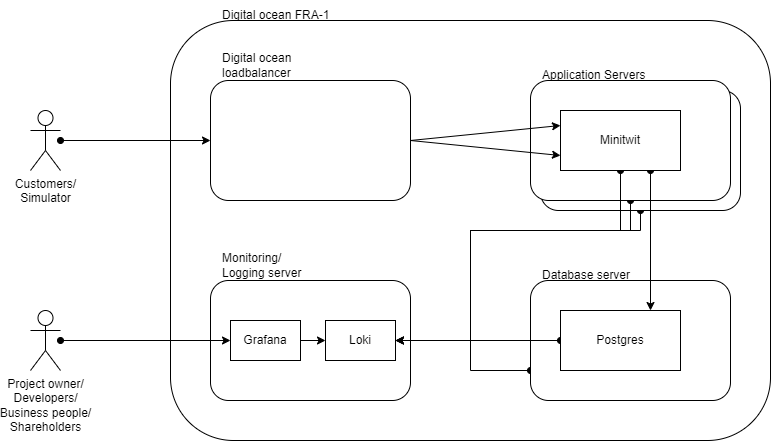
\includegraphics[width=150mm]{images/diagrams/Overview.png}
    \caption{Image of server deployment}
    \label{fig:ServerDeployment}
\end{figure}

To access each of the services and enable the option to use \gls{tls}, there have been configured \gls{dns} records to each of the services, with sub domains to the domain "thomsen-it.dk". The configuration can be seen in \autoref{tab:DnsOverview}


\begin{table}[!ht]
\centering
\begin{tabular}{|l|l|}
\hline
Domain                                                                                                              & Server(s)               \\ \hline
\begin{tabular}[c]{@{}l@{}}thomsen-it.dk\\ www.thomsen-it.dk\end{tabular}                                           & Managed Loadbalancer \\ \hline
database.thomsen-it.dk                                                                                              & Database Server      \\ \hline
\begin{tabular}[c]{@{}l@{}}grafana.thomsen-it.dk\\ prometheus.thomsen-it.dk\\ monitoring.thomsen-it.dk\end{tabular} & Monitoring Server    \\ \hline
\end{tabular}
\captionsetup{justification=centering,margin=1cm}
\caption{\gls{dns} record overview}
\label{tab:DnsOverview}
\end{table}

All the servers have been configured to redirect traffic from port 80 to port 443 and the Nginx reverse proxy on the servers terminates \gls{tls} traffic \cite{deployment_nginx_config}.

\subsection{Design and architecture of of the ITU-MiniTwit system}
% Tænker dette er high level abstraction docker containers view
% Tænker dette er selv code infrastruktur
The code follows the onion architecture pattern seen in  \autoref{fig:onion_architecture}. This pattern has been chosen to easily separate segments of the code.


\begin{figure}[!ht]
    \centering
    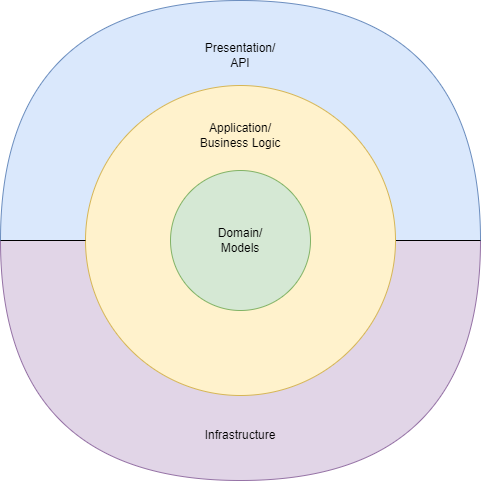
\includegraphics[width=80mm]{images/diagrams/ApplicationOverview.png}
    \captionsetup{justification=centering,margin=1cm}
    \caption{Onion architecture}
    \label{fig:onion_architecture}
\end{figure}


The presentation layer accepts the incoming REST web requests and translates them to method invocations to the application layer. The application layer calls the domain layer and makes sure that the business logic and rules are kept/maintained for each call to the database layer and returned to the presentation layer. The communication between the different layers are depicted in \autoref{fig:SystemDesign}.

\begin{figure}[!ht]
    \centering
    \captionsetup{justification=centering,margin=1cm}
    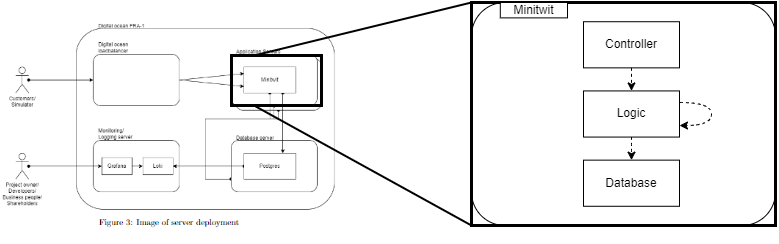
\includegraphics[width=\linewidth]{images/diagrams/system-design-version2.drawio.png}
    \caption{System design of Minitwit Application}
    \label{fig:SystemDesign}
\end{figure}


\subsection{Dependencies of the ITU-MiniTwit system}

%\todo{Christian, Use power linux magix}
% All dependencies of your ITU-MiniTwit systems on all levels of abstraction and development stages.
%That is, list and briefly describe all technologies and tools you applied and depend on.

One of the first important choices were choosing a programming language and suitable web framework as can be seen documented in \href{https://github.com/DevelOpsITU/MiniTwit/issues/33}{\#33}. Here the language Golang and web framework Gin were selected. For package management in Golang, the \href{https://github.com/DevelOpsITU/MiniTwit/blob/main/go.mod}{"go.mod" file} contains all the packages that the project needs, and any indirect packages. These are maintained by Go's own package manager. A dependency graph can be seen in Appendix \ref{app:gomod_dependencies}.

For docker images, the team has based the Go application on an official docker image called "golang:bullseye", which is maintained by the "Docker community"\cite{docker_go_image}. The rest of the docker image dependencies are maintained by the respective project maintainers and are: "postgres:13.5, prom/prometheus:v2.33.5, grafana/grafana:8.4.3, fluent/fluent-bit:1.9.0-debug, nginx:1.15-alpine, grafana/loki:2.4.2", which can be seen the "docker-compose.yaml"\cite{github_minitwit_dockercompose} file.

For hosting, provisioning and management of VM's, the group choose to use Vagrant and the hosting provider DigitalOcean (DO), which both offers services like docker registry, -databases, -Kubernetes and managed apps like Grafana for visualization. None of these services were used however, since the group saw it against the idea of avoiding "Vendor-locking" and makes "Infrastructure-As-Code" harder to make vendor independent. However the team did give in, when the task of scaling came and setting up a managed load balancer just seemed easier to do\href{https://github.com/DevelOpsITU/MiniTwit/issues/174}{\#174}. 

Lastly the group depend on Github both for version control and Github Action for Continuous Integration and pushing to Dockerhub. 


\subsection{Important interactions of subsystems}
% Think that Helge should take over our spot. Crosslevels of abstractions like minitwit and the database.
Figure \ref{fig:interactions} shows the interactions between different services, the developer and the user. Code is developed on individual developer's computers and is pushed and pulled from and to the different GitHub repositories. From a configured CI pipeline code is pulled from the Minitwit repository, tested and build into docker images, uploaded to Docker Hub. The developer manually runs scripts from the ServerDeployment repository to update the droplets in Digital Ocean.\\
The user accesses the application through a managed load balancer that sends the user to either running application droplet, which each has a reverse proxy, that finally sends traffic to the minitwit application.\\
The monitoring server interacts with the other droplets, by pulling information from them. Only the two application droplets interact with the database.
\begin{figure}[H]
    \centering
    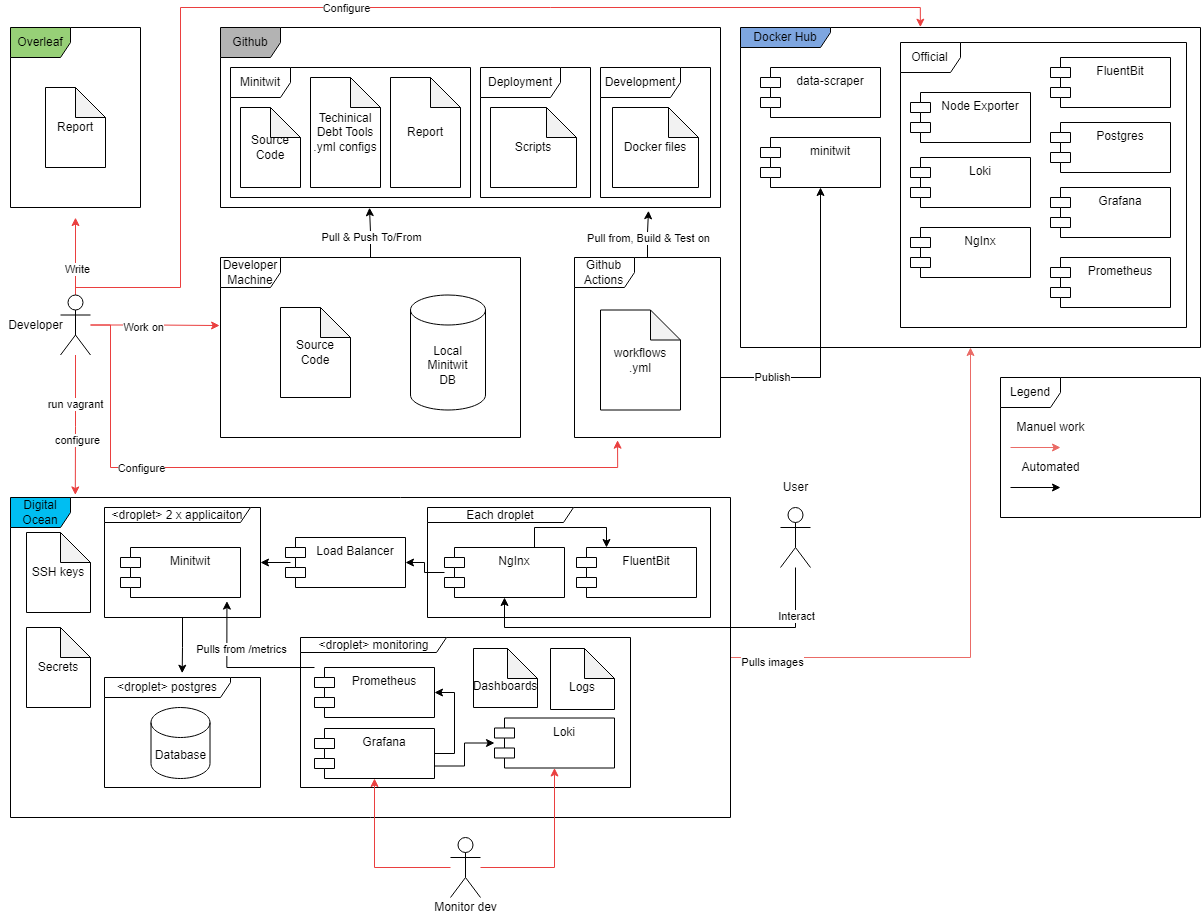
\includegraphics[width=\linewidth]{images/diagrams/Interactions.png}
    \caption{Interactions between services}
    \label{fig:interactions}
\end{figure}


\subsection{Current state of the ITU-MiniTwit system}
%Describe the current state of your systems, for example using results of static analysis and quality assessment systems.
The current state of the system shown by the static analysis and quality assessment tools can be seen in \autoref{fig:CodeQuality}

\begin{figure}[!ht]
    \centering
    \captionsetup{justification=centering,margin=1cm}
    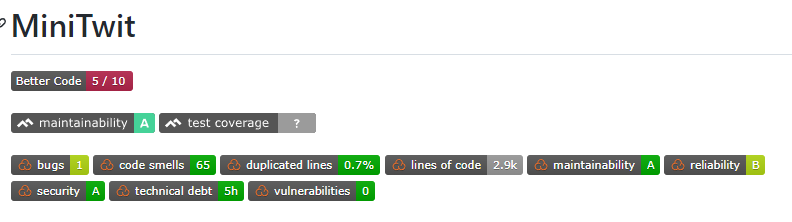
\includegraphics[width=\linewidth]{images/code_quality.png}
    \caption{Code Quality of Minitiwit Application (Source: own image)}
    \label{fig:CodeQuality}
\end{figure}
From these quality metrics, it can be seen that the results of Sonarcloud returns mostly positive quality, with a bunch of code smells. However, from these code smells only 24 are critical, yet these are not of great importance. \\
Compared to Sonarcloud, Better Code results in a much lower score due to a several reasons including too many lines in single functions, code duplication and low test coverage.

\subsection{Chosen project license}
%Finally, describe briefly, if the license that you have chosen for your project is actually compatible with the licenses of all your direct dependencies.
In order to decide on a project licence, we had to audit whether it would be compatible with the licenses in our direct dependencies. In our case, these dependencies were Go binaries and it was difficult to find a general-purpose licence scanner for our project (for example, the tool "scan-code", which was proposed by our guest lecturer, did not work in our case). However, after doing some research, we decided that "Lichen" would be the best option (we also tried out "GoLicence", but we couldn't make it work). As can be seen in issue \href{https://github.com/DevelOpsITU/MiniTwit/issues/134}{\#113}, we used "Lichen" to count the number of different direct licences our Go project contained. In total, our project contained 31 MIT, 6 Apache -2.0, 5 BSD-3-Clause and finally one BSD-2-Clause licence. Consequently, we choose an Apache-2.0 licence, since this is compatible with MIT, BSD-2 and 3-Clause. This decision stem from the fact that our project include Apache-2.0 licences and since Apache-2.0 is less permissive than MIT, BSD-2 and 3-Clause, we need to match the Apache-2.0 licence, which is more restrictive than the three aforementioned licences. As a final note, we also tried other scanning tools for licence detection, but these lie outside the scope of this chapter.
% Syntes det er godt at nævne de værktøjer vi bruger til at nå frem til den data vi bruger til at bestemme lisens.


%OBS: CHECK THAT:
% all the weekly tasks (those listed in the schedule) you include the corresponding information.
% All tech choices and decisions that we have made in the tasks at the end of each session has been documented 